\documentclass[11pt]{article}

\usepackage{polish}
\usepackage[utf8]{inputenc}
\usepackage{url}
\usepackage{hyperref}
\usepackage{multicol}
\usepackage{geometry}
\usepackage{fancyhdr}
\usepackage{graphicx}
\usepackage{enumitem}

\setlist[itemize]{noitemsep, topsep=5pt}
\geometry{a4paper,total={170mm,257mm},left=20mm,top=20mm}

\graphicspath{ {../} }

\pagestyle{fancy}
\rhead{Raport I }
\lhead{}
\cfoot{\thepage}

\newcounter{coun}[section]
\newenvironment{coun}[1][]{\refstepcounter{coun}\par\medskip
{\noindent\textbf{\thecoun #1. }}\leftskip=0em\rightskip=0em }{\par\medskip}

\begin{document}
\title{Raport I \\  (środowisko agenta i reprezentacja wiedzy)}
\author{Marcin Woźniak \\ Filip Izydorczyk \\ Hubert Wrzesiński \\ Przemysław Fierek}
\maketitle
\vspace{20}
Repozytorium: \url{https://github.com/linux923344/autonomiczny_saper/}} \\

\coun {Zaprojektowanie diagramu klas.}\\
\begin{center}
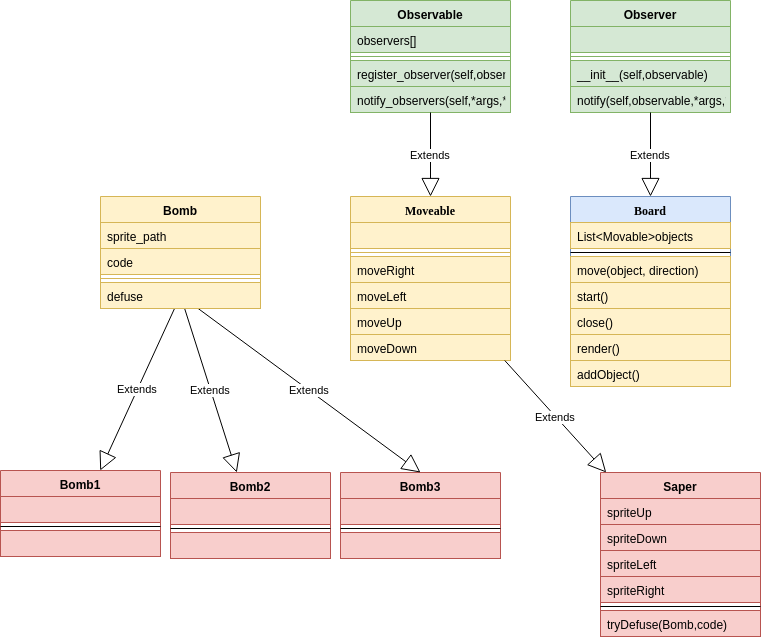
\includegraphics[scale=0.6]{logika.png}
\end{center}
\coun {Na podstawie diagramu, została stworzona klasa główna oraz jej podklasy.}
\coun {Został stworzony szablon planszy razem z umieszczonymi na niej bombami. }\\
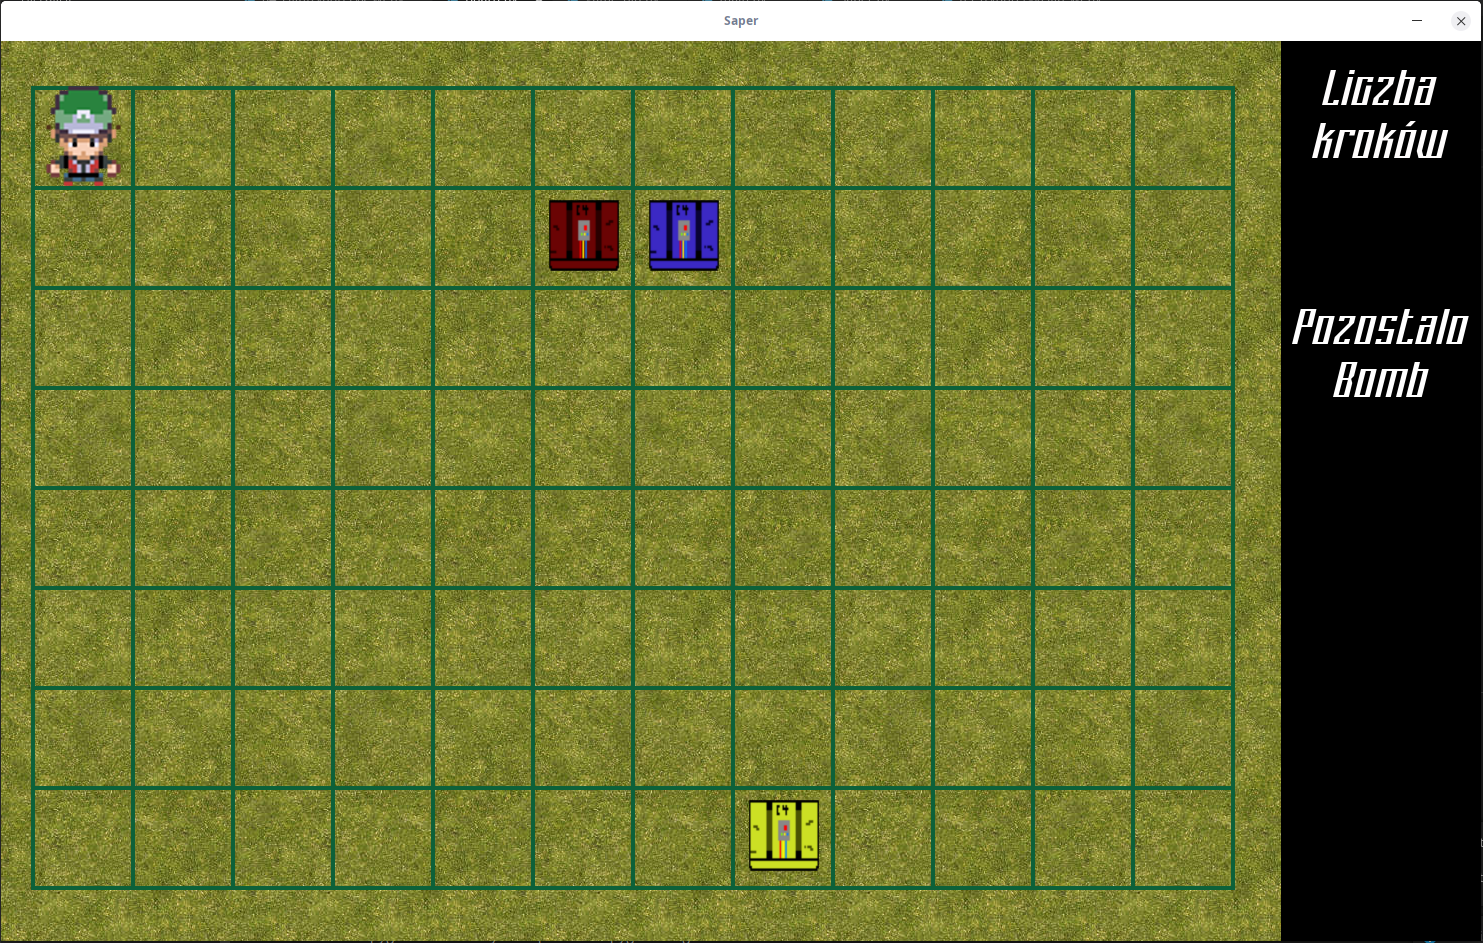
\includegraphics[scale=0.5]{plansza.png}
\end{document}

